\section{Validazione e Fase di Test}
Al fine di creare pagine il più possibile accessibili da parte delle diverse tipologie di utente sono stati utilizzati strumenti automatici di validazione e di testing, oltre ai test eseguiti manualmente, per avere un'interpretazione corretta e accessibile da parte di tutti i browser indifferentemente dai dispositivi utilizzati.

\subsection{Strumenti per la validazione}
Tutte le pagine e il relativo codice sono stati sottoposti alla validazione attraverso i seguenti strumenti:
\begin{itemize}
	\item Total Validator, disponibile per il download al sito ufficiale \url{https://www.totalvalidator.com/};
	\item validatore W3C per il CSS, disponibile online al link \url{https://jigsaw.w3.org/css-validator/};
	\item validatore W3C per l'HTML, disponibile online al link \url{https://validator.w3.org/};
	\item Colour Contrast Analyser per l'analisi dei colori utilizzati, disponibile per il download al sito ufficiale italiano \url{https://www.webaccessibile.org/} o disponibile online al link \url{https://webaim.org/resources/contrastchecker/}.
\end{itemize}
\textbf{Nota}: la validazione del codice HTML è stata fatta incollando direttamente il codice sorgente prodotto dalle pagine PHP nel validatore, in modo tale da poter validare tutto quel codice non presente nelle pagine in HTML.

\subsection{Strumenti per la fase di test}
L'intero sito è stato testato manualmente sui seguenti browser da desktop:
\begin{itemize}
	\item Safari;
	\item Microsoft Internet Explorer/Edge;
	\item Microsoft Edge (beta) basato su Chromium;
	\item Google Chrome;
	\item Mozilla Firefox.
\end{itemize}
Sono stati effettuati test manuali anche per la versione mobile utilizzando differenti browser mobile. In particolare sono stati utilizzati i dispositivi:
\begin{itemize}
	\item Asus Zenfone 3 Max, con sistema operativo Android 7.0;
	\item Blackview bv9000, con sistema operativo Android 7.1.1;
	\item Huawei P20 Lite, con sistema operativo Android 9.0;
	\item Apple iPhone XS, con sistema operativo iOs 13.4.1.
\end{itemize}
L’usabilità del sito web rimane invariata, essendo quest’ultimo responsive, anche se presenta layout o comportamenti differenti per cause che dipendono dal sistema operativo. Per tale motivo la fase di test sui dispositivi mobile è stata eseguita minuziosamente e parallelamente alla fase di test per il desktop.

\subsection{Test per l'accessibilità}
A partire dalla struttura in HTML si è cercato di rendere più efficiente la navigazione del sito, per permettere a tutte le categorie di visitatori di accedere a tutti i contenuti nel miglior modo possibile.

Un occhio di riguardo si è avuto per tutte quelle persone che presentano difficoltà visive. Si è scelto di mantenere sempre un alto contrasto tra il colore di sfondo ed il colore delle scritte, per non intaccare la leggibilità delle ultime, sono stati inseriti gli attributi tabindex, gli span di lingua, gli attributi alt per facilitare la lettura dei contenuti con l'uso di screen reader.\\

In particolare sono stati eseguiti dei test che simulano la visione con diverse tipologie di daltonismo. Le immagini, di seguito riportate, sono state generate con l'utilizzo del simulatore Coblis, disponibile online al link \url{https://www.color-blindness.com/coblis-color-blindness-simulator/}.\\
\\
\captionof{figure}{Homepage del sito}
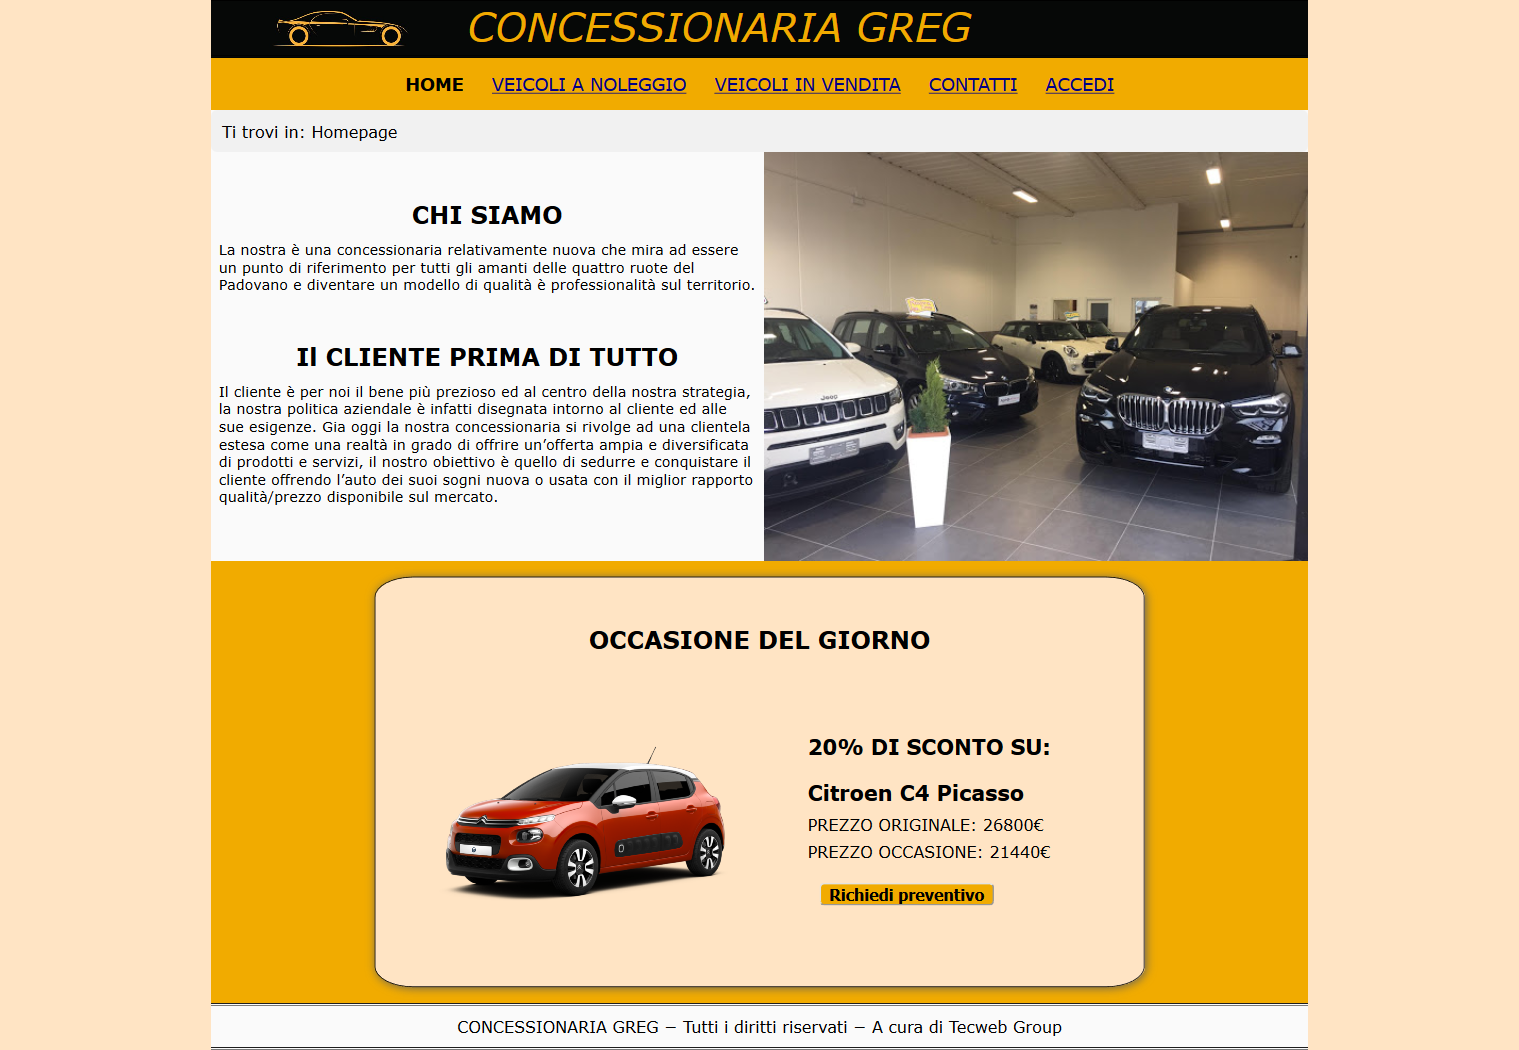
\includegraphics[width=8pc]{./img/homepage-normal.png} 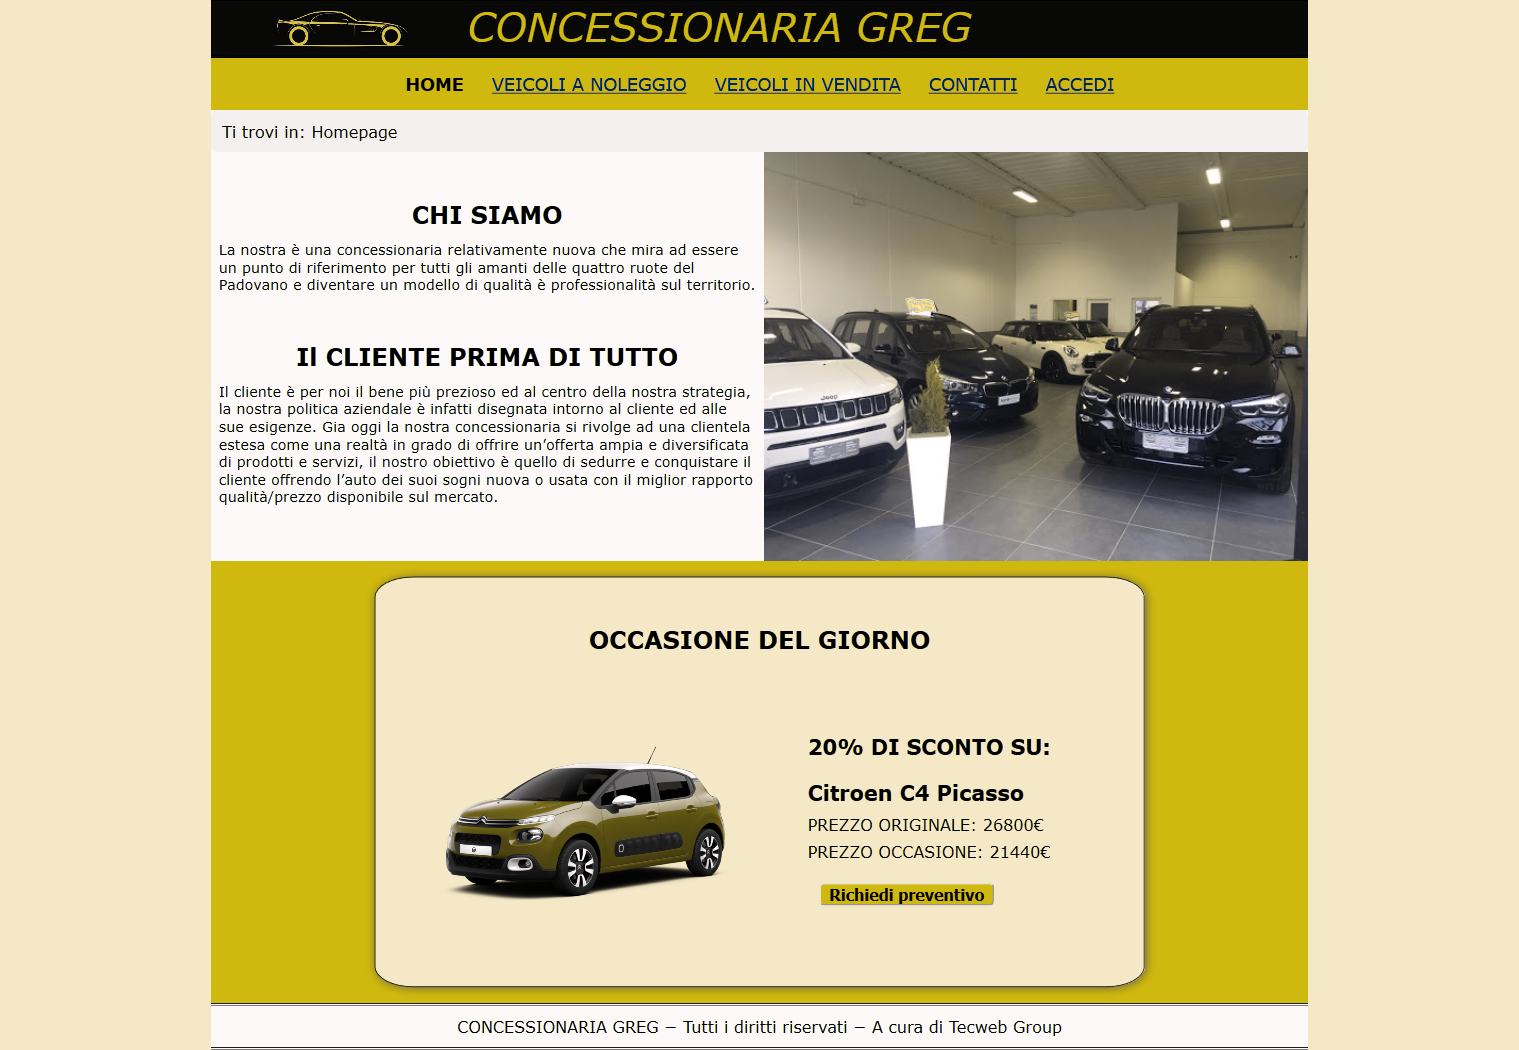
\includegraphics[width=8pc]{./img/homepage-protanopia.png} 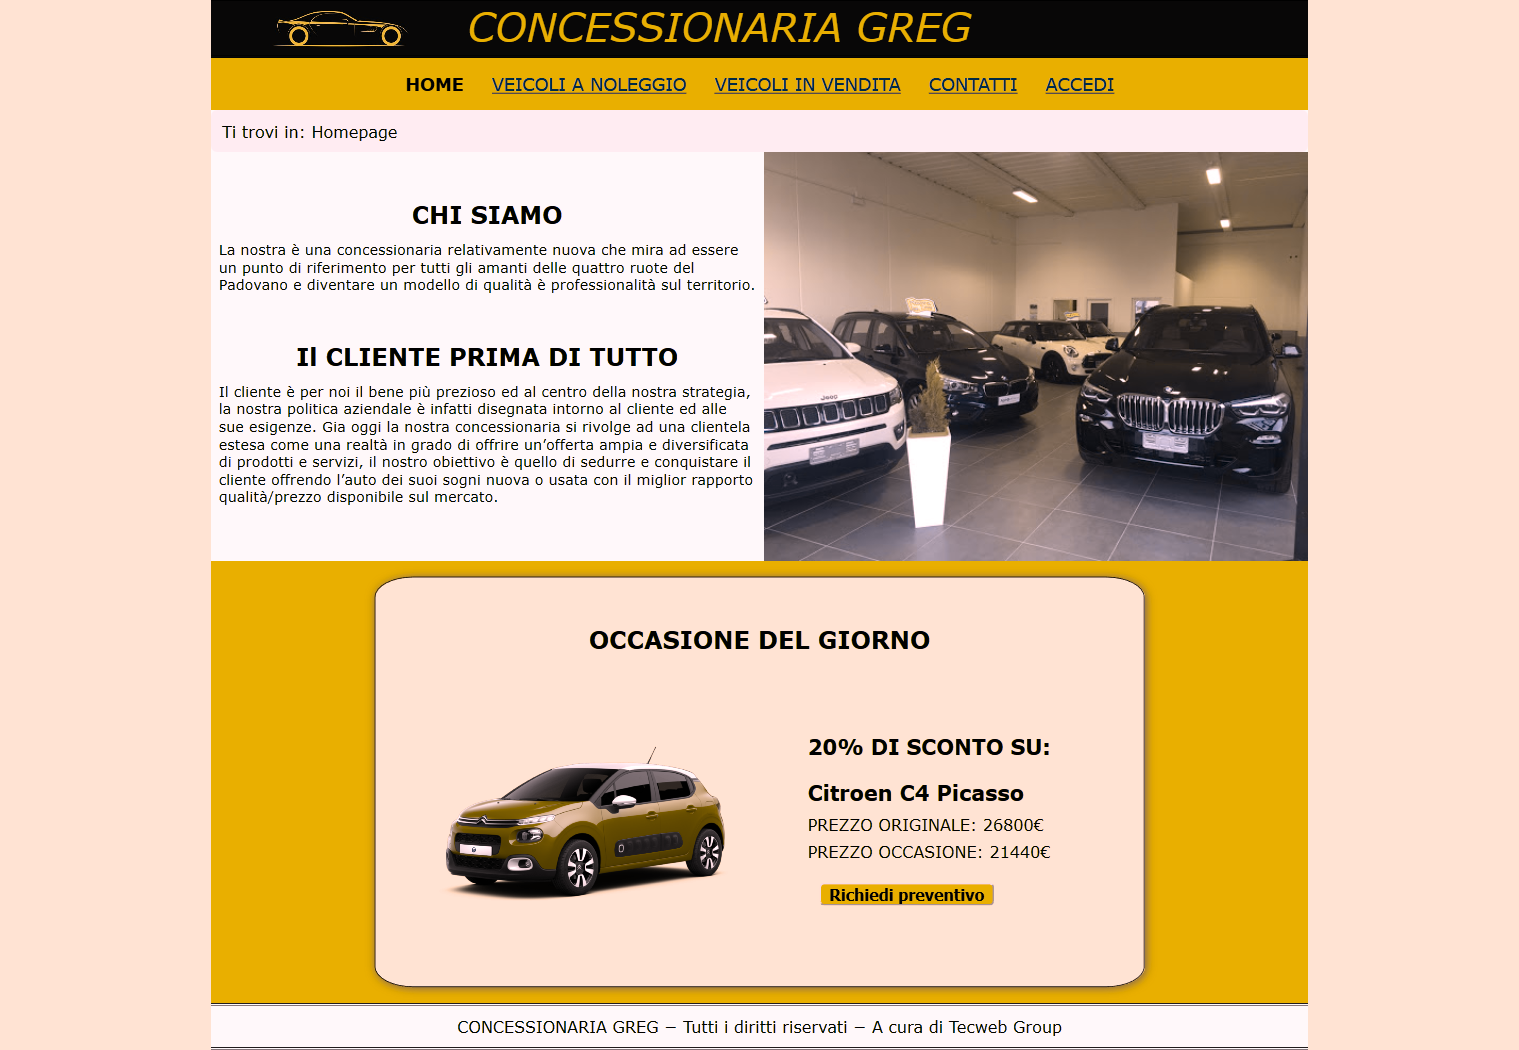
\includegraphics[width=8pc]{./img/homepage-deuteranopia.png} 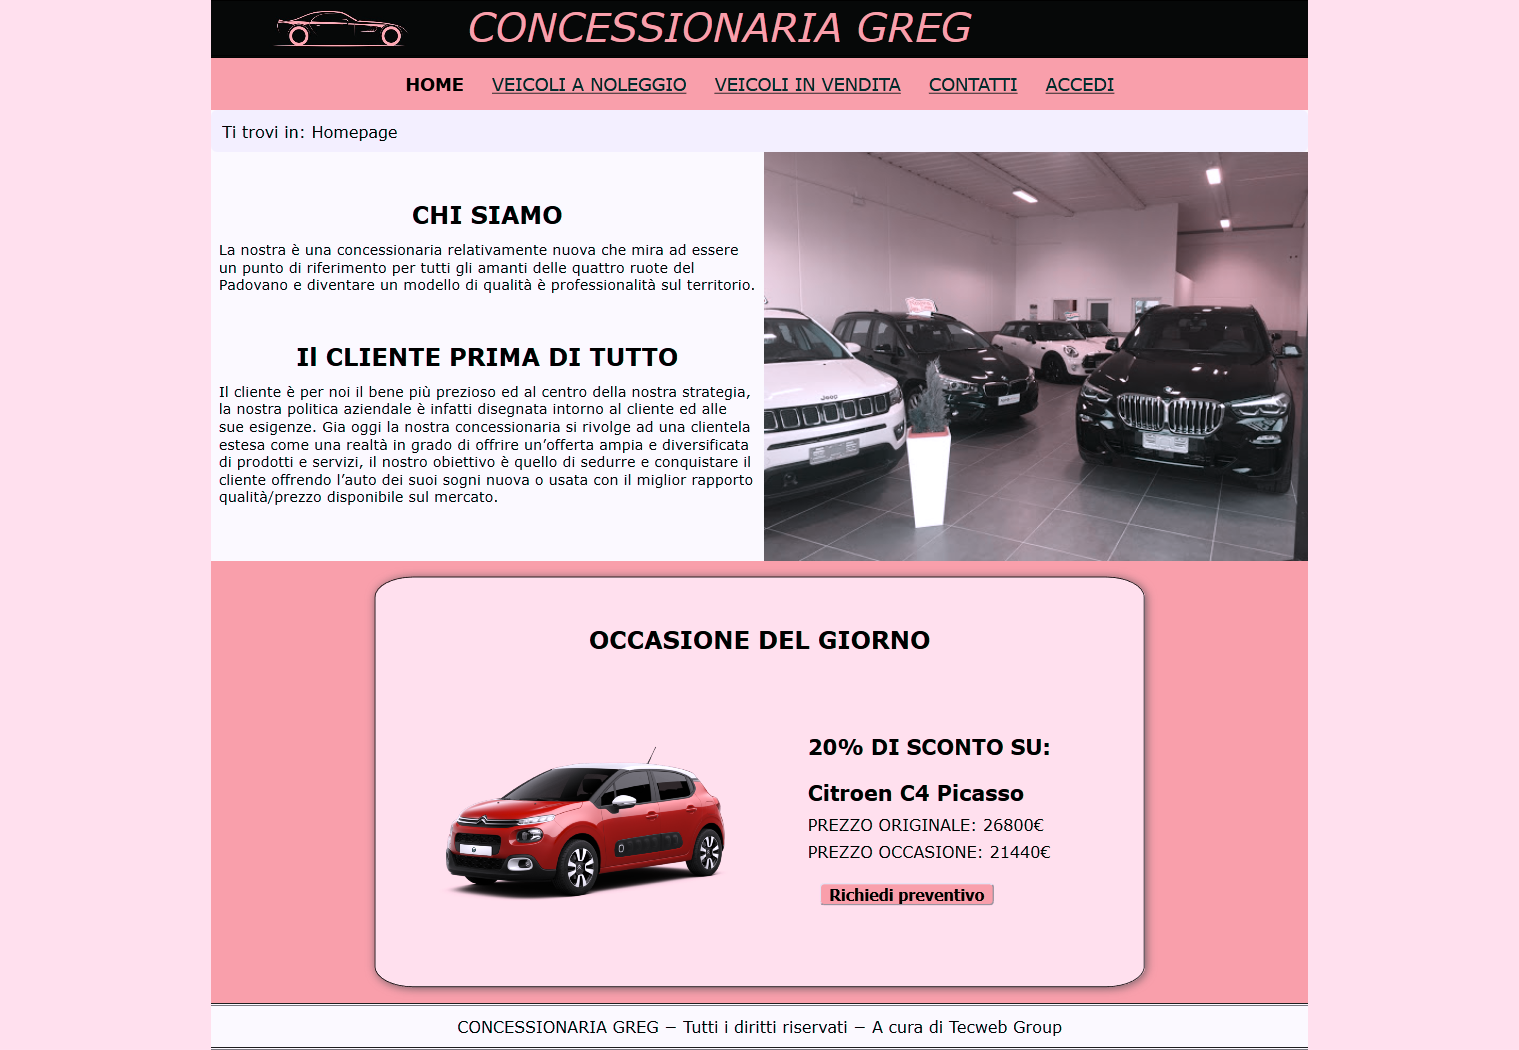
\includegraphics[width=8pc]{./img/homepage-tritanopia.png}\\

\captionof{figure}{Pagina di accesso all'area personale con messaggio di errore}
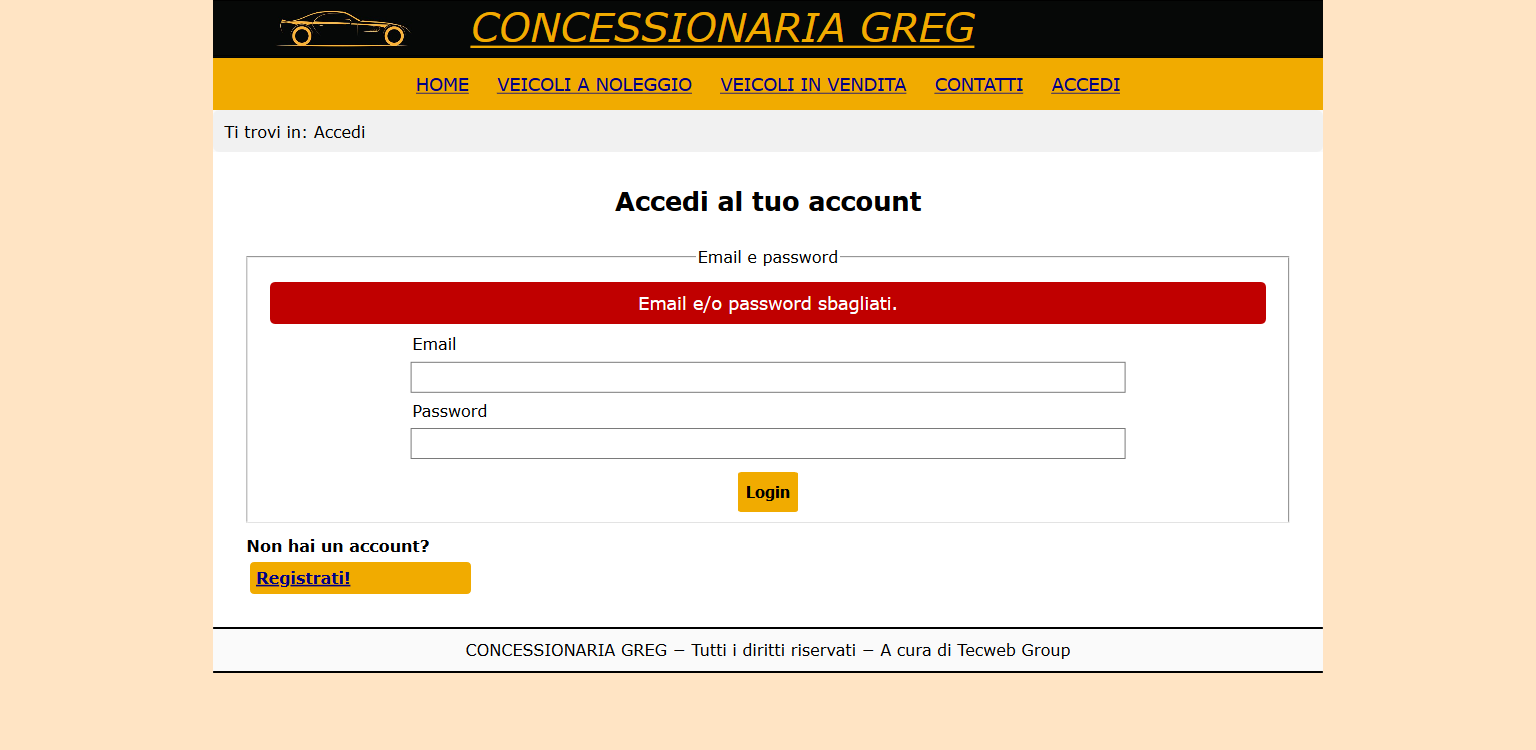
\includegraphics[width=8pc]{./img/pagina_accesso_errore-normal.png} 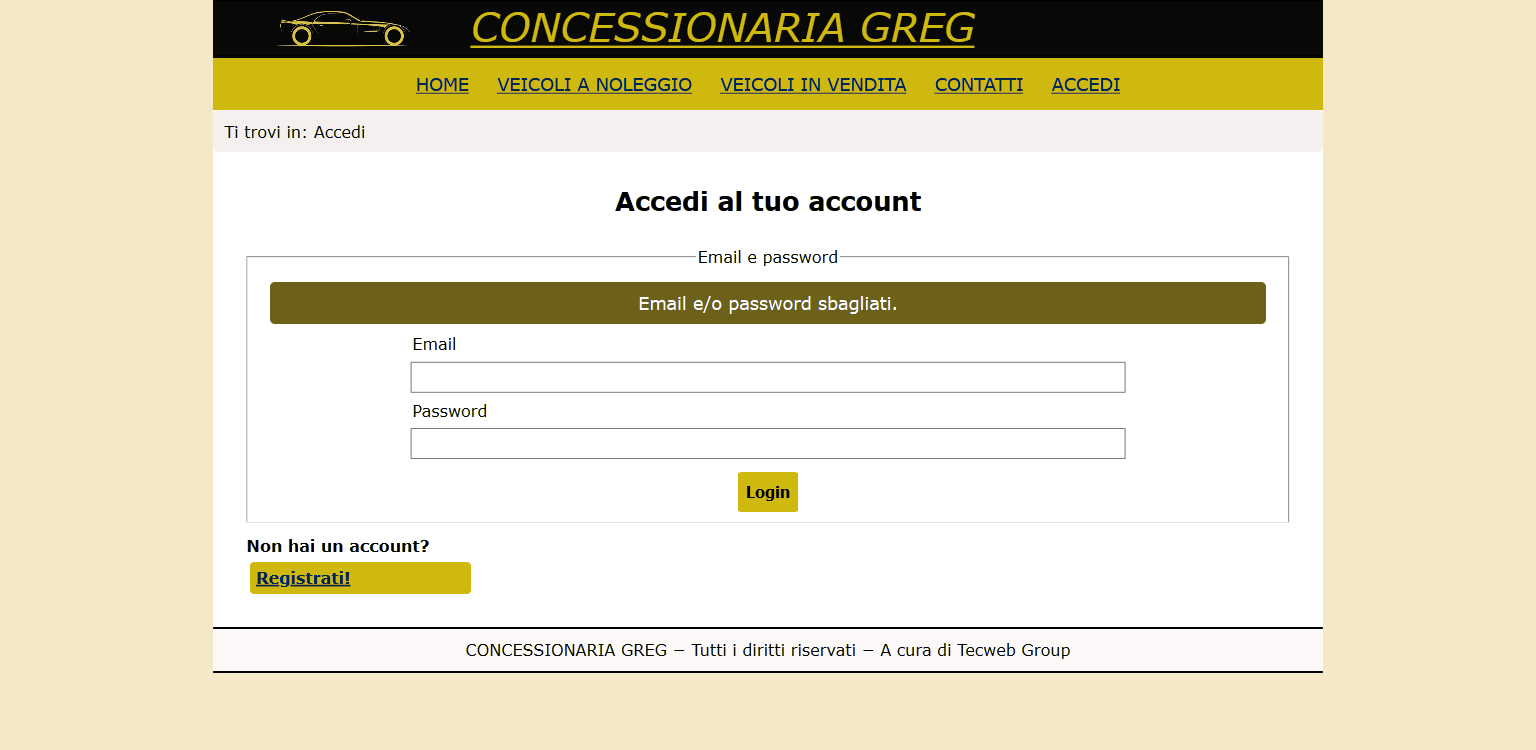
\includegraphics[width=8pc]{./img/pagina_accesso_errore-protanopia.png} 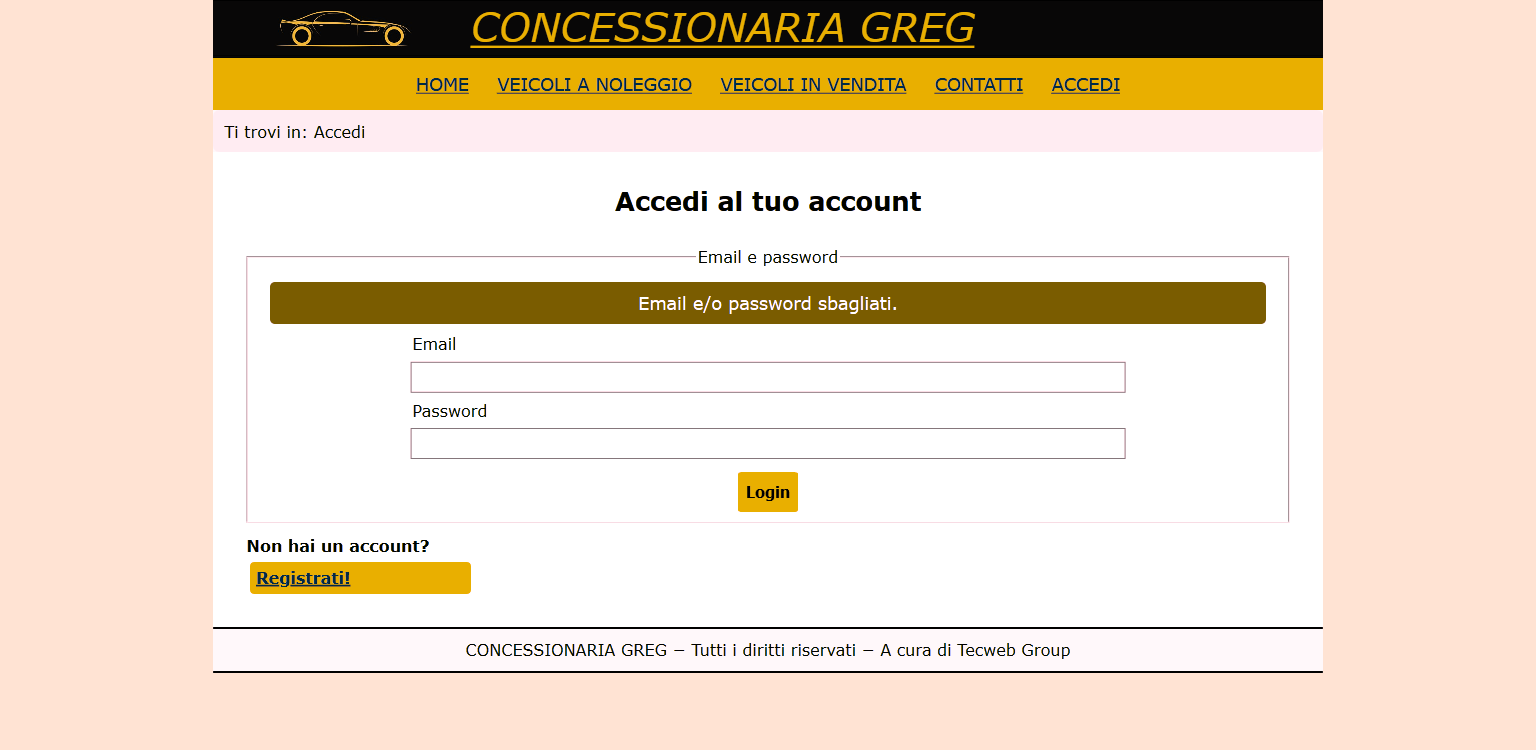
\includegraphics[width=8pc]{./img/pagina_accesso_errore-deuteranopia.png} 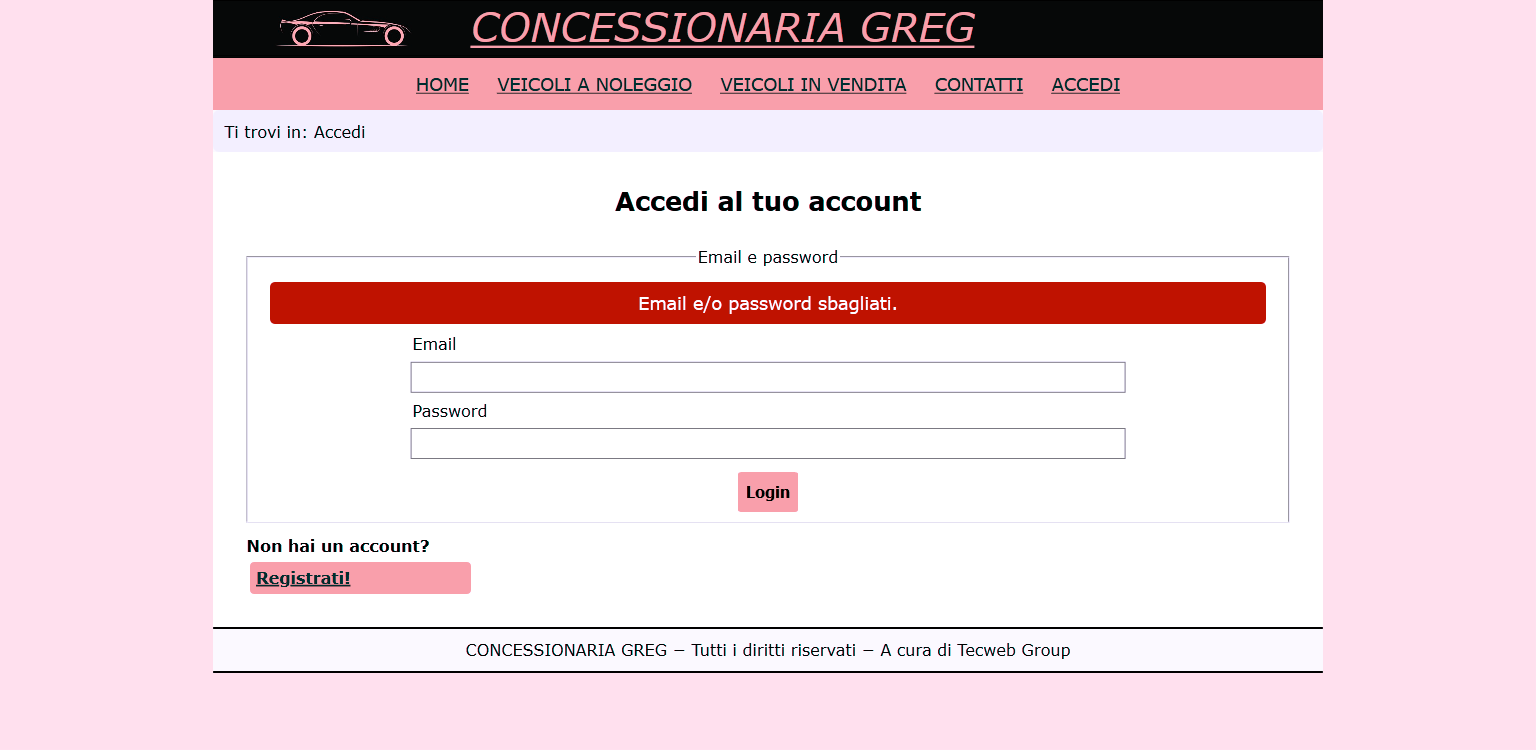
\includegraphics[width=8pc]{./img/pagina_accesso_errore-tritanopia.png}\\

\captionof{figure}{Pagina con la lista di tutti i veicoli in vendita con messaggio di successo}
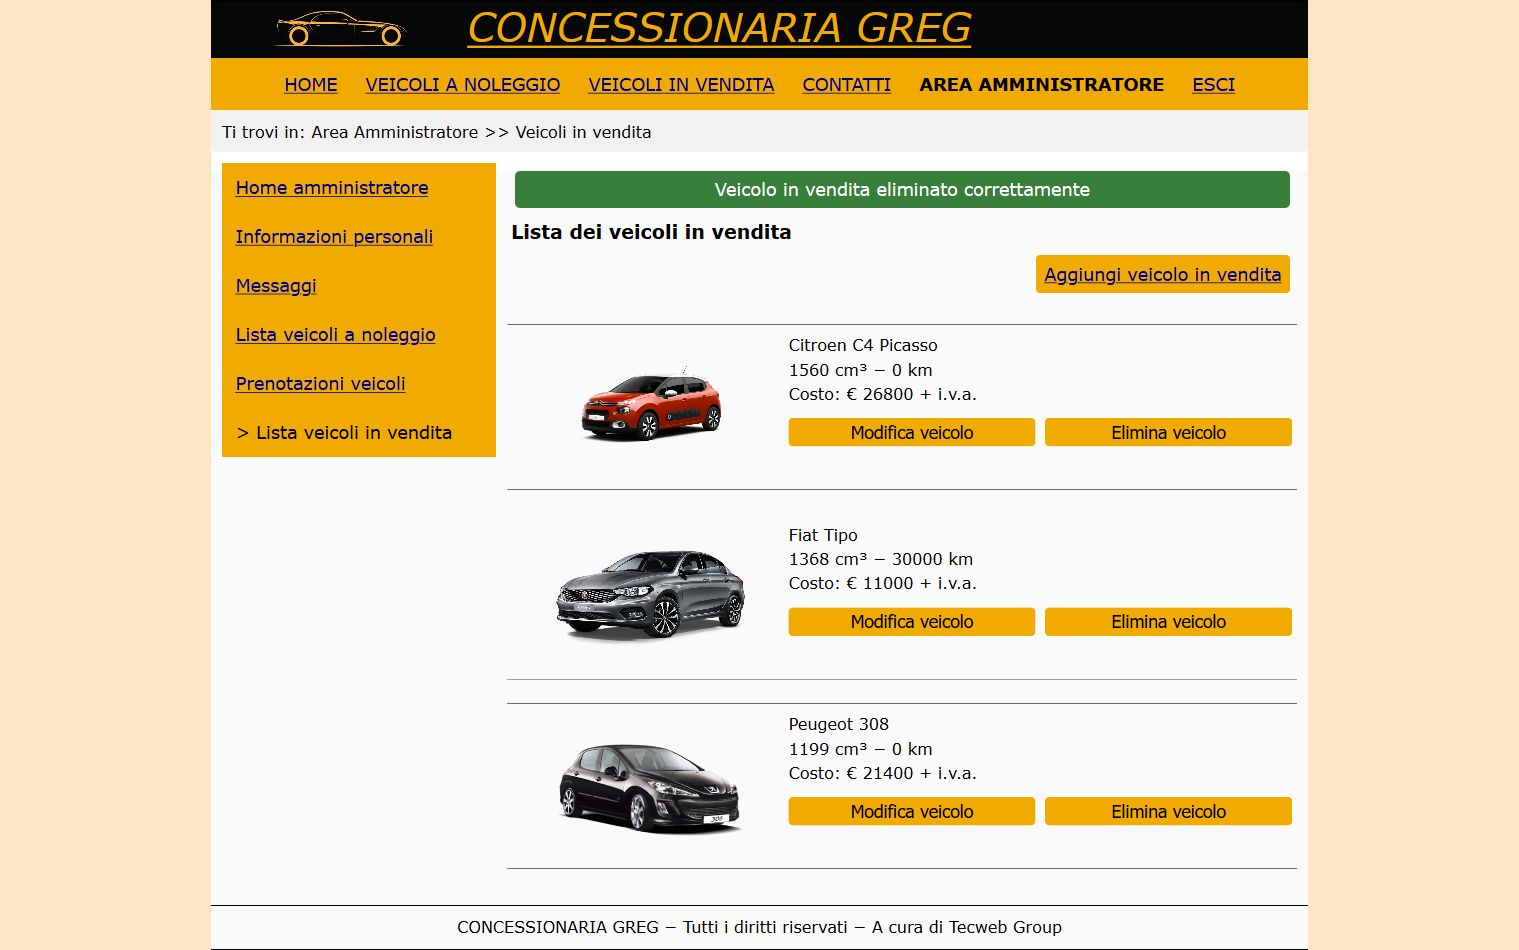
\includegraphics[width=8pc]{./img/pagina_lista_veicoli_vendita-successo-normal.png} 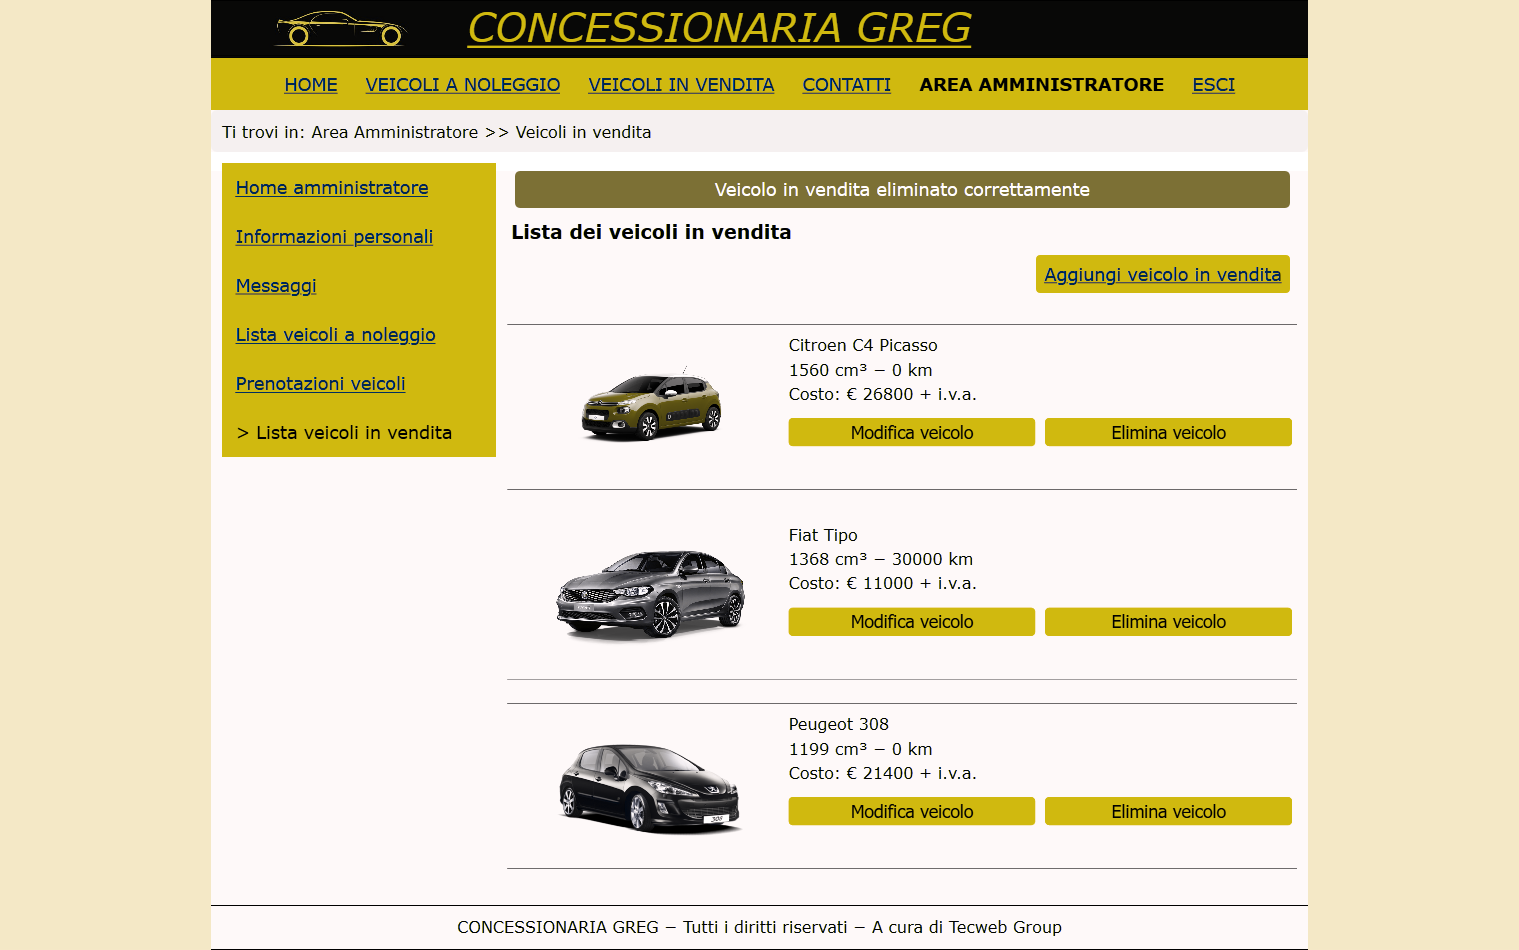
\includegraphics[width=8pc]{./img/pagina_lista_veicoli_vendita-successo-protanopia.png} 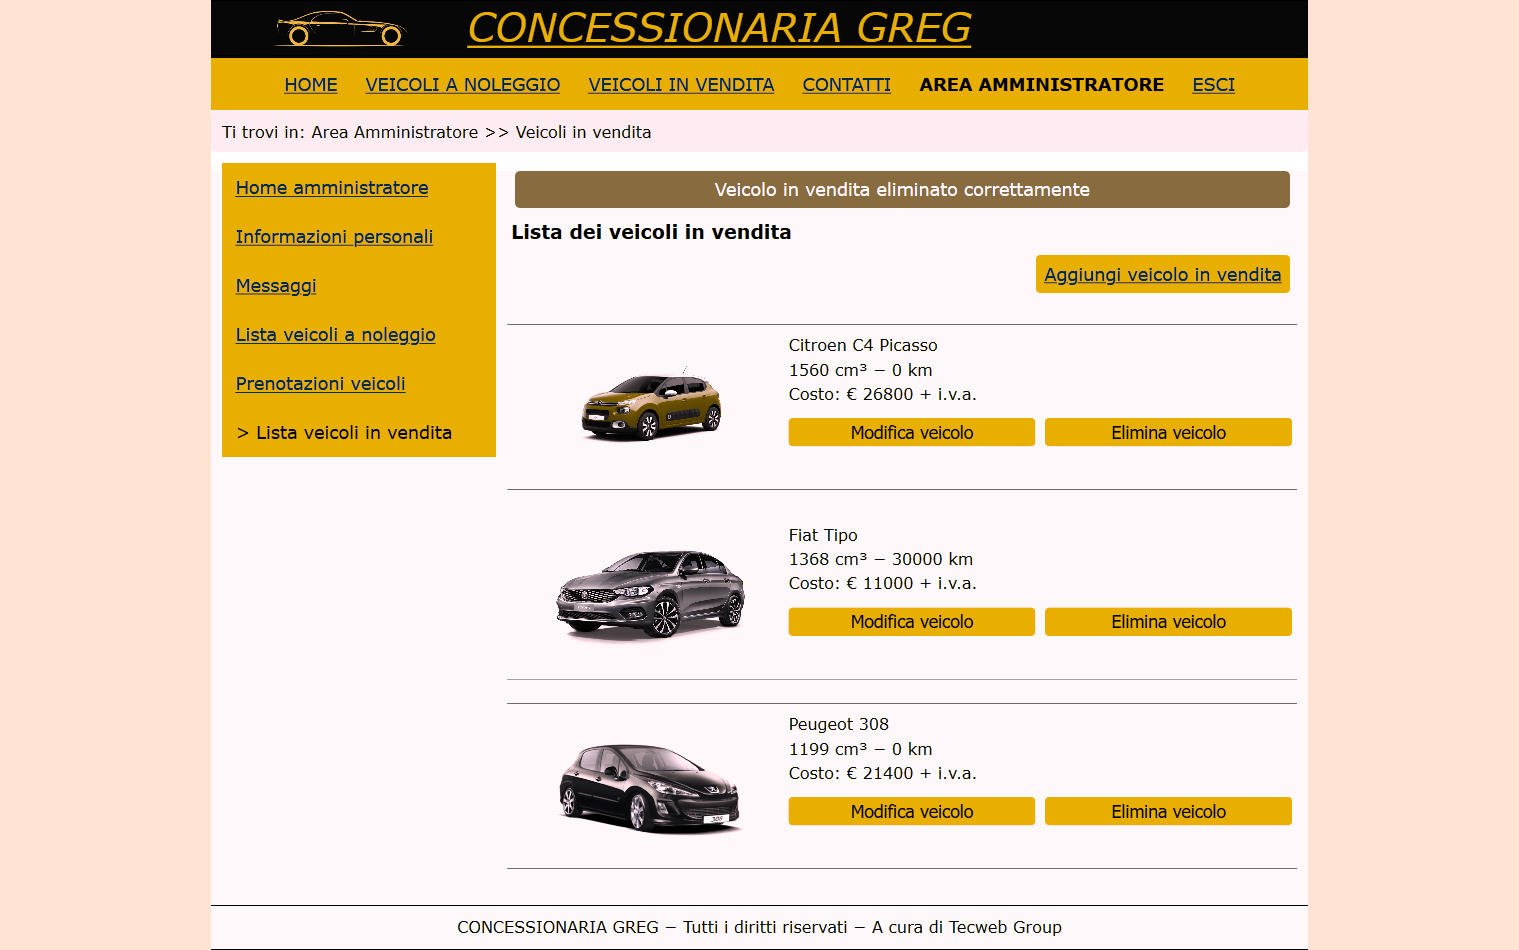
\includegraphics[width=8pc]{./img/pagina_lista_veicoli_vendita-successo-deuteranopia.png} 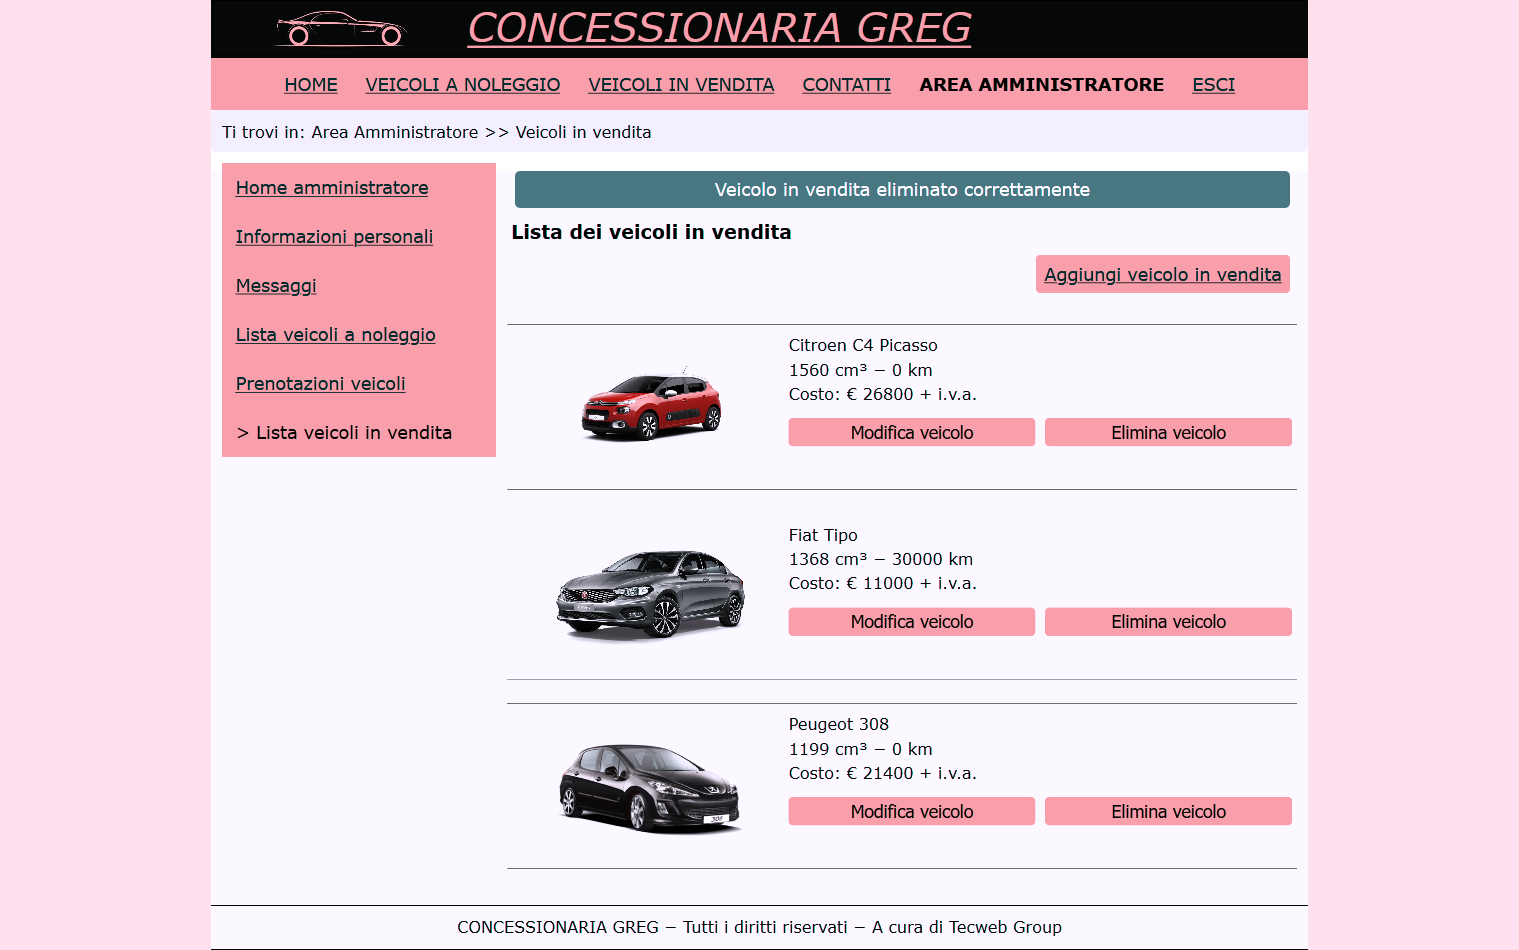
\includegraphics[width=8pc]{./img/pagina_lista_veicoli_vendita-successo-tritanopia.png}\\

\captionof{figure}{Pagina per la modifica delle informazioni personali dell'utente registrato}
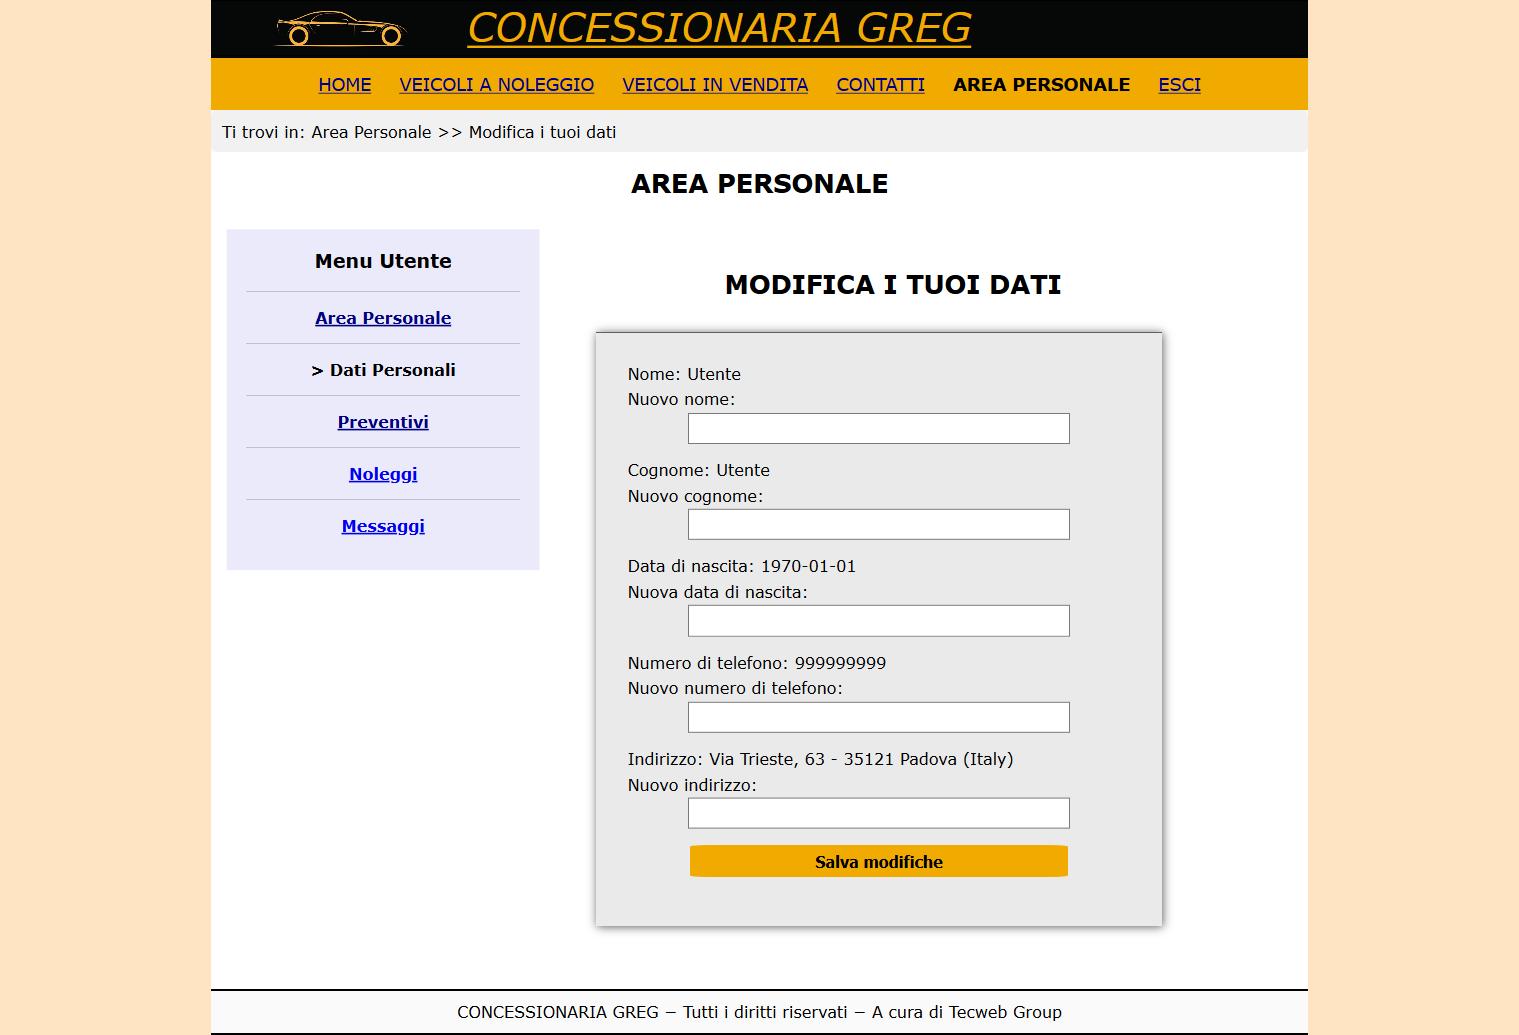
\includegraphics[width=8pc]{./img/pagina_modifica_info_utente-normal.png} 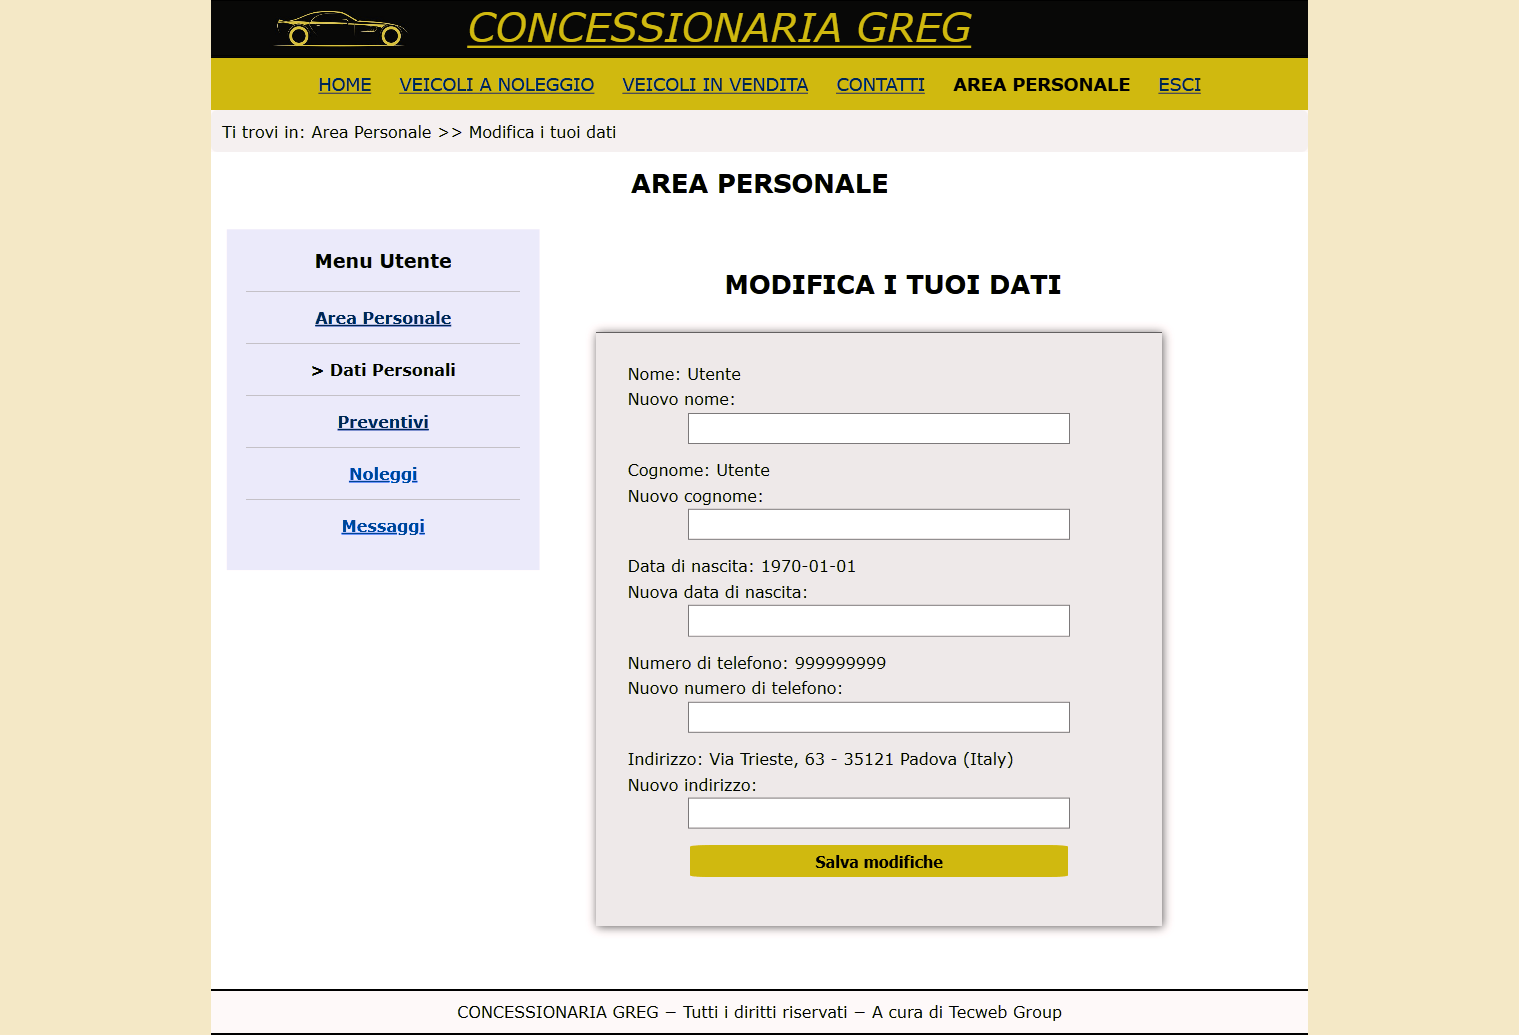
\includegraphics[width=8pc]{./img/pagina_modifica_info_utente-protanopia.png} 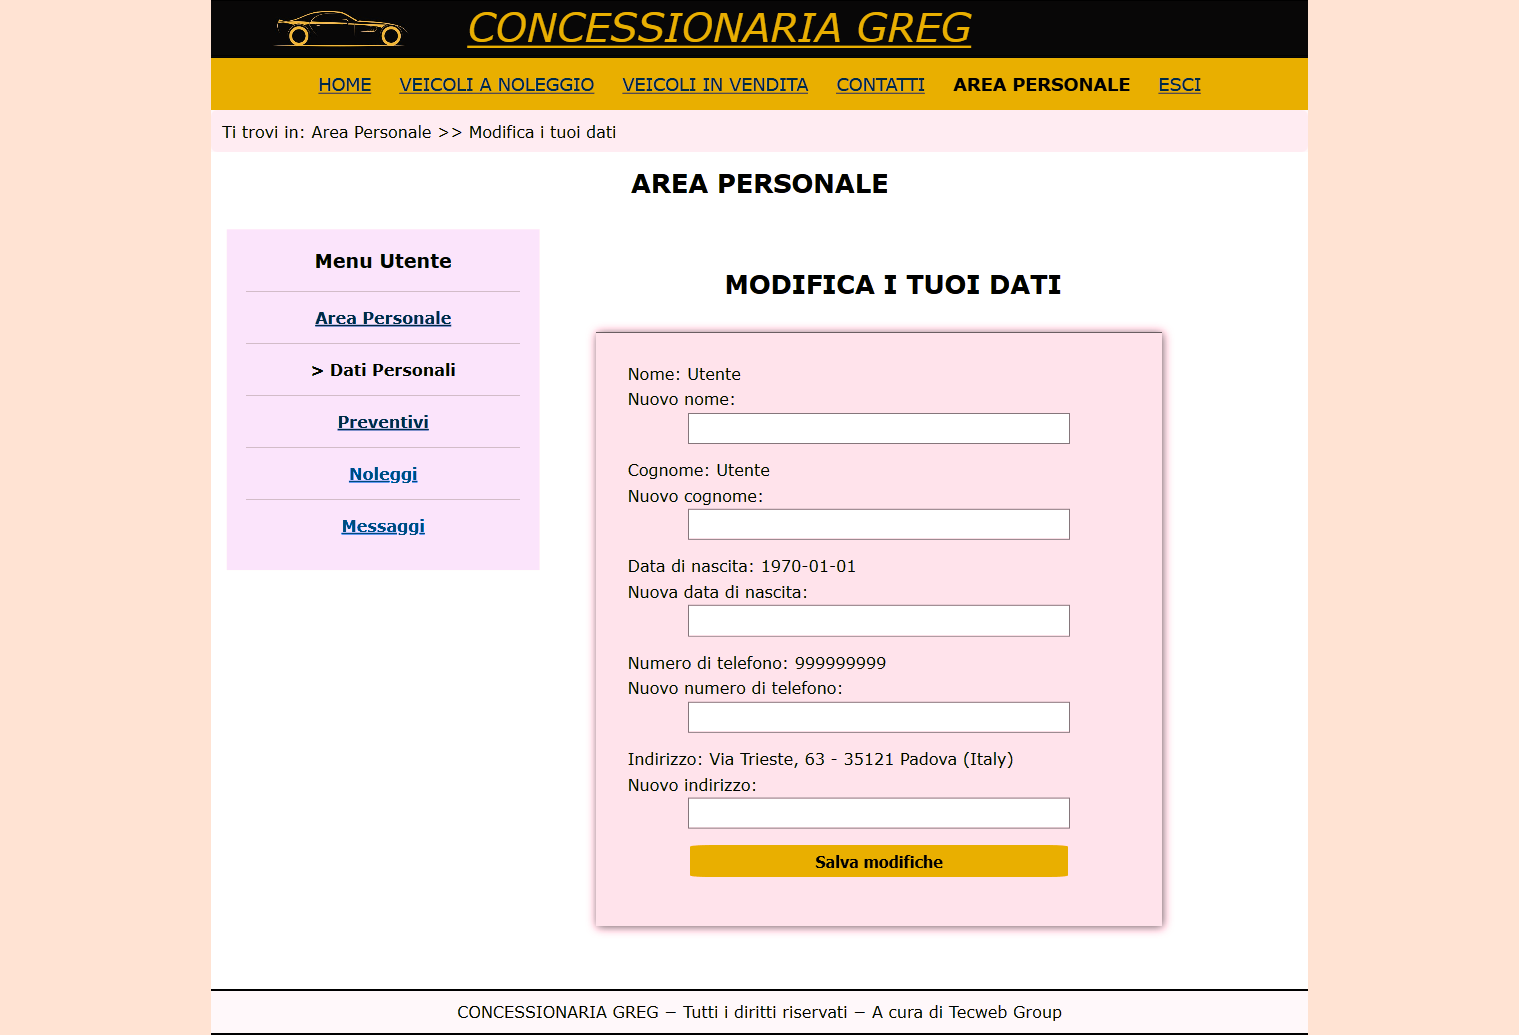
\includegraphics[width=8pc]{./img/pagina_modifica_info_utente-deuteranopia.png} 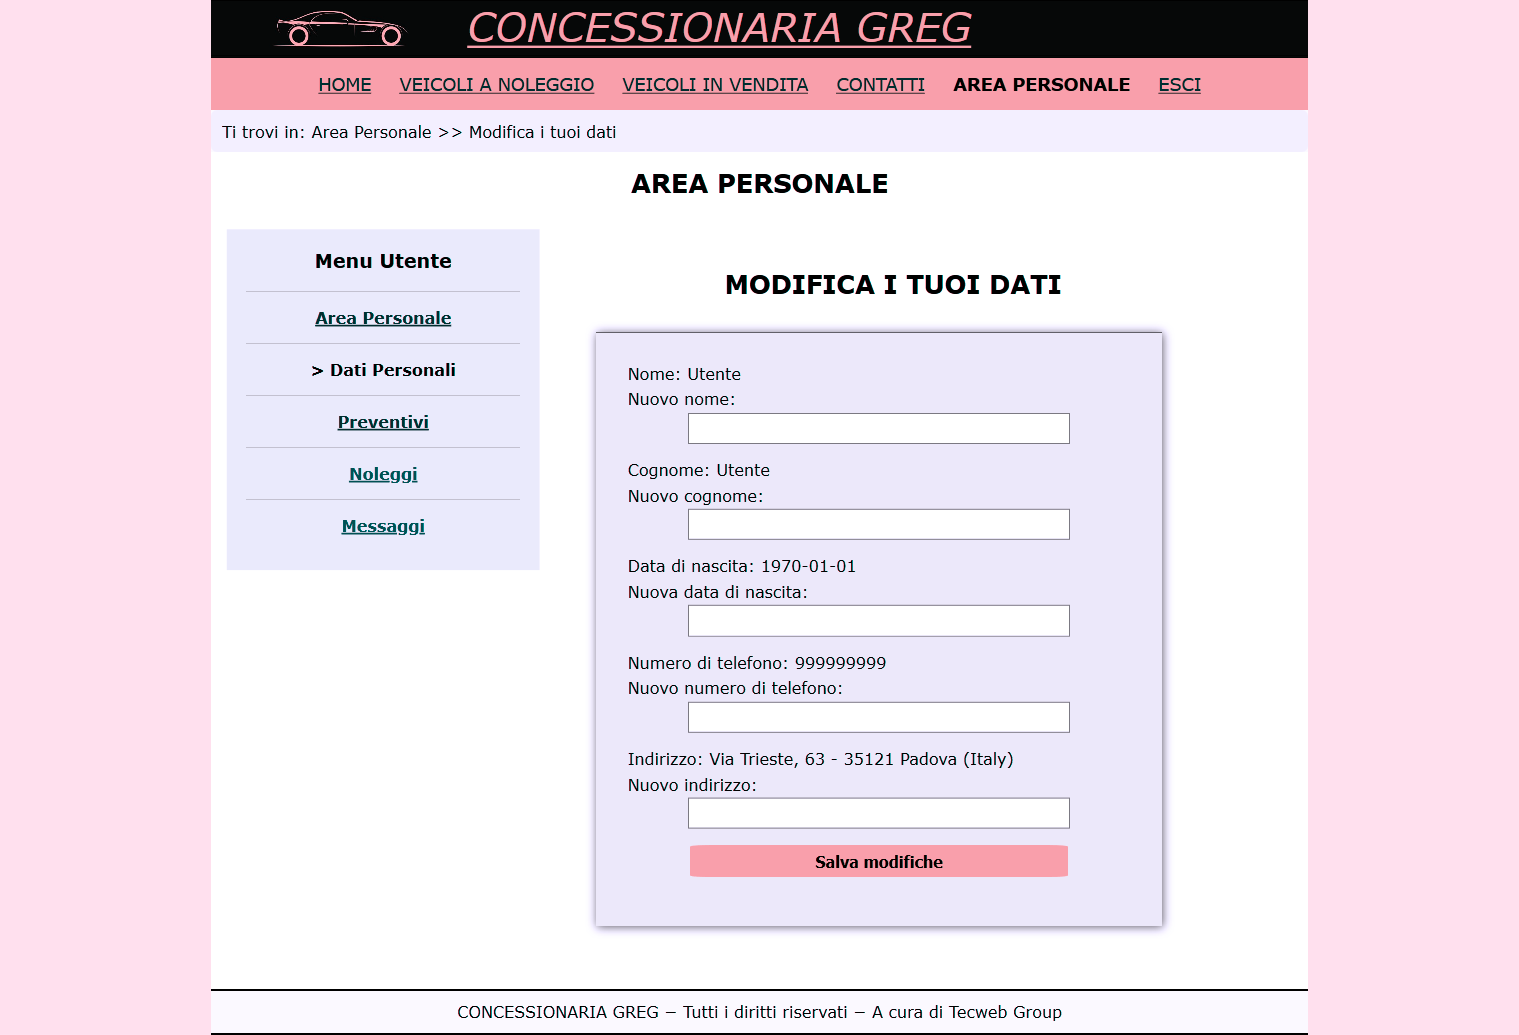
\includegraphics[width=8pc]{./img/pagina_modifica_info_utente-tritanopia.png}\\

\pagebreak
